\chapter{Prototype Design}

The aim of this project is to design and develop a prototype digital library for Māori language users to meet the needs of Māori language users for book retrieval, borrowing and return functions, and to improve the library experience for Māori language users. The prototype library is aimed at the Maori speaking community around the world, including Maori teachers, students, parents and general users\cite{Pixso官网新0:online}.

Māori language is one of the official languages of New Zealand's indigenous Maori people and is an important part of New Zealand's cultural and social development. In order to promote the heritage and development of the Maori language, the prototype digital library will provide Maori language users with rich and diverse Maori language book resources to facilitate their online reading and learning, and will also make a positive contribution to Maori language education and cultural heritage\cite{Discover30:online}.

\section{Design principles and methodology}

The design of the digital library prototype will follow the following principles:

User-centered: The project will focus on user needs, user experience and satisfaction, to provide users with efficient and convenient humanized services.

Diversity and inclusion: The digital library prototype will provide a variety of resources from the rich and diverse Māori language culture, covering different areas and topics, embracing a variety of cultures and ideologies, and reflecting the diversity of Māori culture.

\section{Prototype introduction}

\subsection{Main interface}

\begin{figure}[htbp]
  \centerline{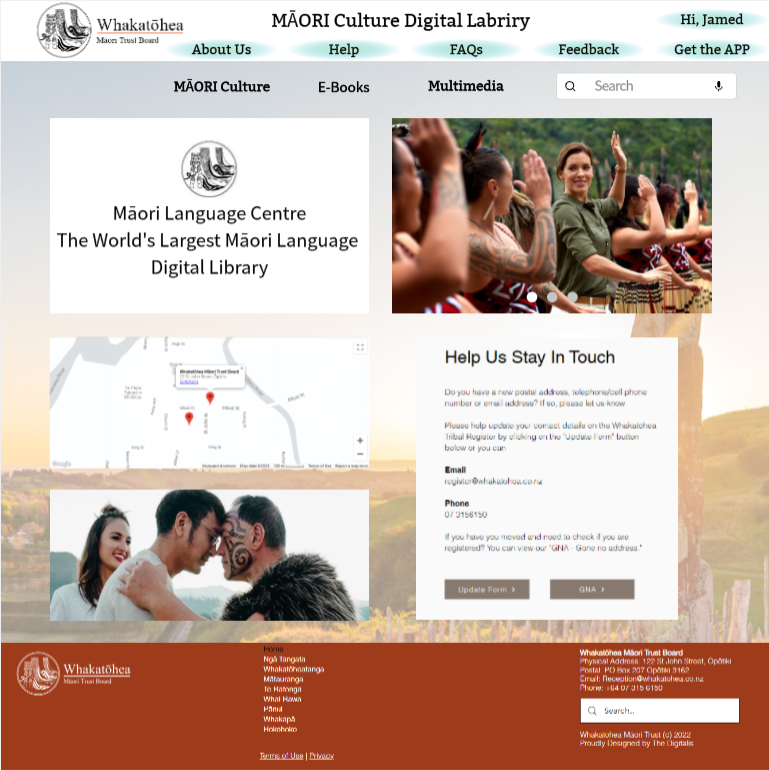
\includegraphics[width=400pt]{images/3-1-1.png}}
  \caption{Main interface}
  \label{fig30}
\end{figure}

After the user logs in, the main interface will show the Māori cultural background, the address of the Maori cultural community, the pictures of the introduction of Maori cultural activities, the links of E-books and multimedia, and the search function of the whole network. Here you can find all the resources we upload and provide, and you can also ask for help to carry out Māori language practice in the community and communicate with other Maori language learners.

\subsection{User interface}

\begin{figure}[htbp]
  \centerline{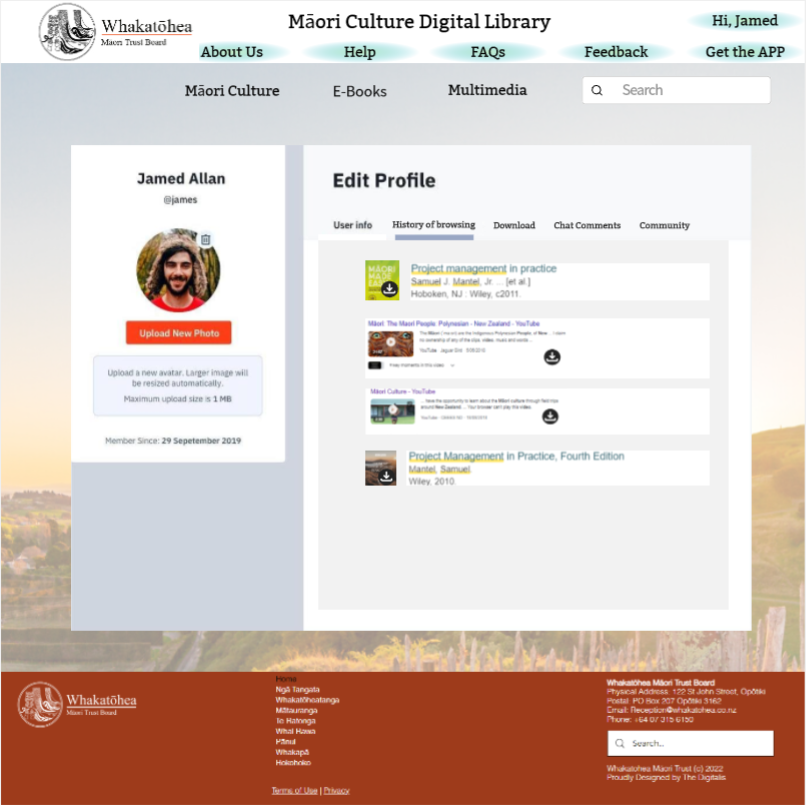
\includegraphics[width=400pt]{images/3-1-2.png}}
  \caption{User interface}
  \label{fig30}
\end{figure}

After the user logs in, The system will record user information, users can modify information through the user interface, view browsing history and like the collection of E-books or multimedia, also can communicate with friends here and view the comments of E-books or multimedia.

\subsection{Māori cultural interface}

\begin{figure}[htbp]
  \centerline{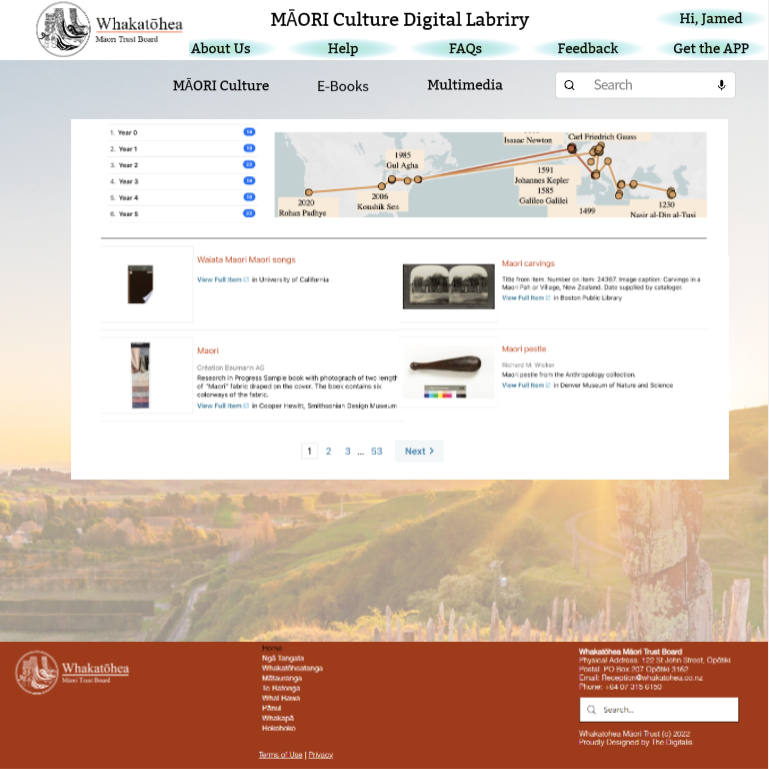
\includegraphics[width=400pt]{images/3-1-3.png}}
  \caption{Māori cultural interface}
  \label{fig30}
\end{figure}

We add a Māori culture interface where users can find all about the development process of Māori culture, migration history and distribution changes, as well as the existing Māori cultural products, which will provide more research channels for current and future learners of Māori culture, from buildings, objects to custom products to show the development process of Māori culture in all aspects\cite{MāoriCul4:online}.

\subsection{E-books browsing interface}

\begin{figure}[htbp]
  \centerline{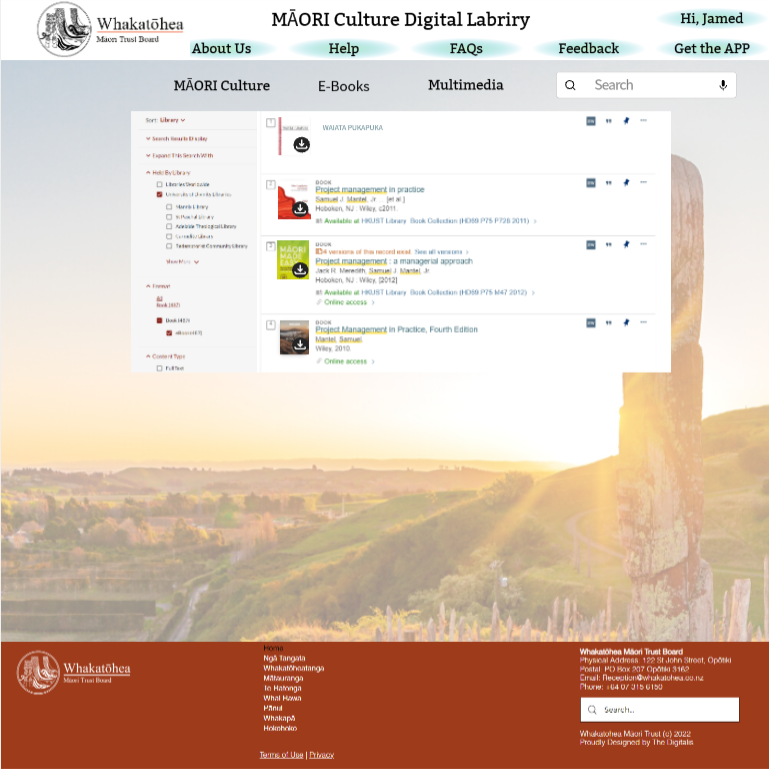
\includegraphics[width=400pt]{images/3-2-1.png}}
  \caption{E-books browsing interface}
  \label{fig30}
\end{figure}

In the E-books browsing interface, users can search related E-books through filters, and all filters we designed include the function of voice input, which can provide convenience for some disabled learners. Typing a keyword in the filter or filtering in the left toolbar will display the relevant E-books.

\subsection{The E-book interface}

\begin{figure}[htbp]
  \centerline{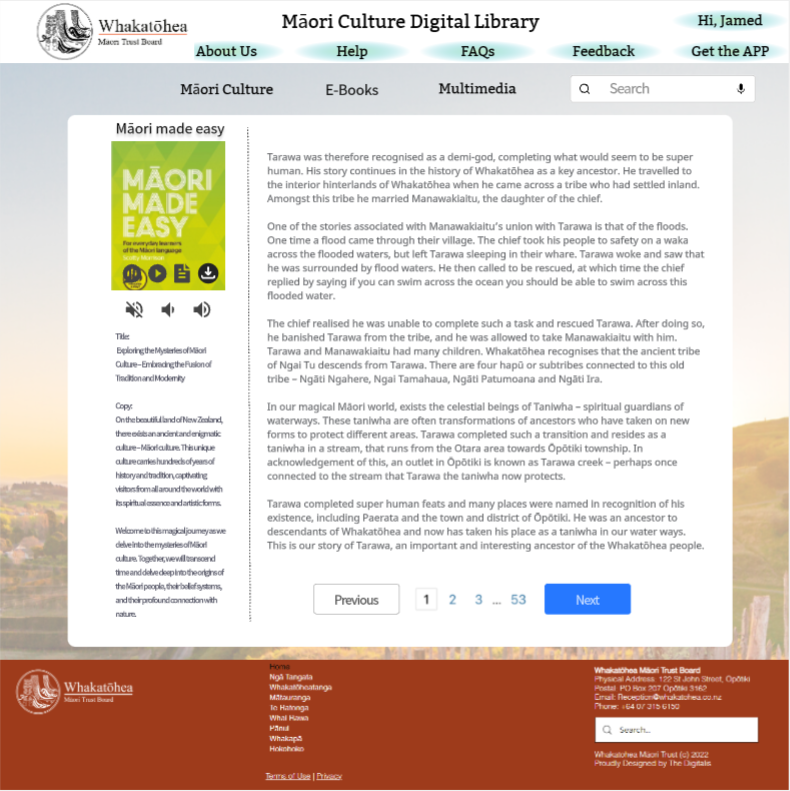
\includegraphics[width=400pt]{images/3-2-2.png}}
  \caption{The E-book interface}
  \label{fig30}
\end{figure}

In the E-books interface, users can read text or listen to E-books through the voice playback function, and provide translation functions for other languages. All resources provided by the e-library are downloadable.

\subsection{Video interface}

\begin{figure}[htbp]
  \centerline{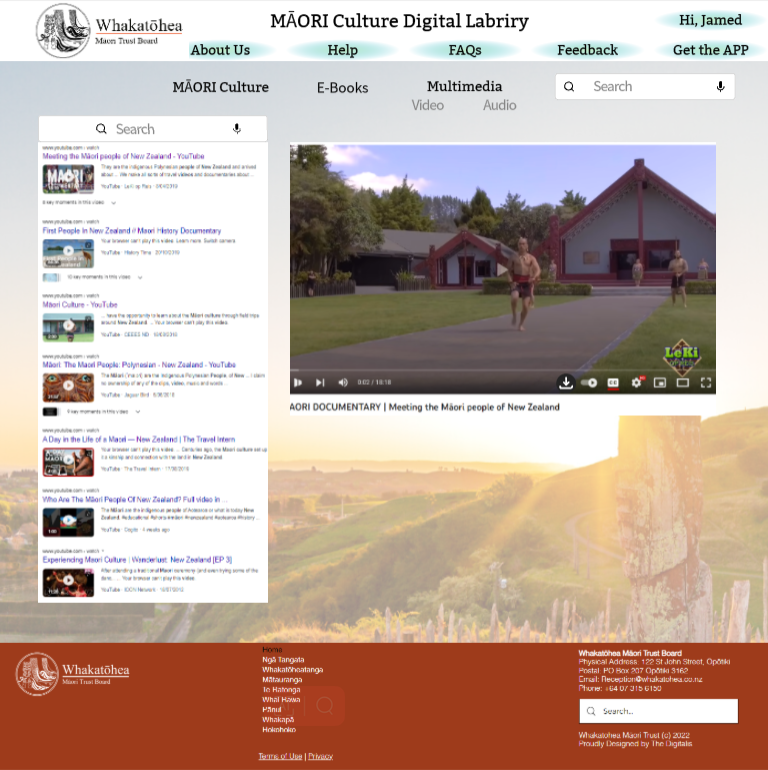
\includegraphics[width=400pt]{images/3-3-1.png}}
  \caption{Video interface}
  \label{fig30}
\end{figure}

In the video interface, users can search related videos by keywords or related words. The filter provides many options such as upload time, picture quality, video duration, and subtitles in other language to facilitate Māori learners to view.

\subsection{Audio interface}

\begin{figure}[htbp]
  \centerline{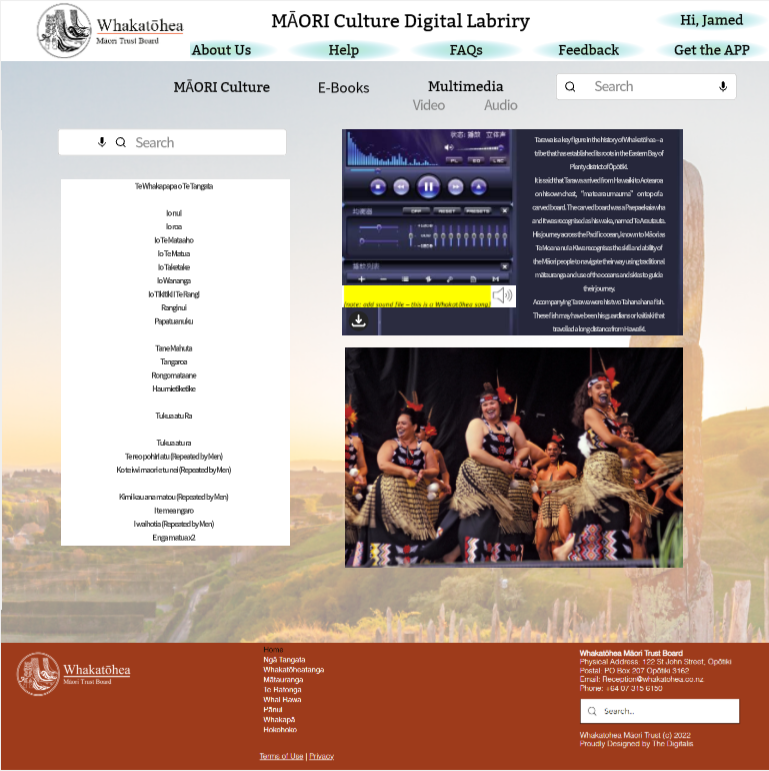
\includegraphics[width=400pt]{images/3-3-2.png}}
  \caption{Audio interface}
  \label{fig30}
\end{figure}

In the audio interface, users can search related audio by the keywords or related words. When playing audio files, subtitles in other languages will be displayed synchronously in the player, and the audio content will be displayed on the left side, which can provide learning convenience for Māori language learners. Audio related videos or pictures are displayed below, which provides a good learning environment for audio learning and deefies learners' memory\cite{MaoriHis64:online}.

\section{Conclusion and Prospect}

Through the design and implementation of this project, the prototype of digital library for Maori users has realized the main functions such as book and multimedia retrieval. The library prototype can provide rich and diverse Maori cultural resources to facilitate users to read and learn online\cite{Māori–Te85:online}.

The designed prototype still has some limitations and shortcomings, including the process of user interface design and interaction can be further optimized, the function of multimedia interface can be more humanized, and the front-end visualization of the library can be more abundant to meet all Maori culture learners for learning.

As technology continues to advance and the Maori language community continues to grow, the digital library prototype needs to be constantly updated and upgraded to meet the changing needs and expectations of its users. At the same time, the digital library will also make greater contributions to the Maori language education and cultural inheritance, promote the inheritance and development of the Maori language, and promote the communication and integration of multiple cultures. We look forward to the Maori Digital library becoming an important learning and communication platform for Maori language users and making greater contributions to the future development of the Maori language community\cite{MaoriCul16:online}.
